\documentclass[a4paper]{article}
\usepackage{amsmath,amssymb,algorithmic,booktabs,bm,caption,cases,csvsimple,enumerate,float,geometry,graphicx,indentfirst,listings,makecell,multirow,setspace,tabularx,titlesec,xcolor}
\captionsetup[figure]{labelsep=period}
\captionsetup[table]{labelsep=period}
\geometry{left=3.5cm,right=3.5cm,top=3.3cm,bottom=3.3cm}
\renewcommand\thesection{\arabic{section}}
\setlength{\parindent}{2em}
\begin{document}
\begin{center}
\huge
\textbf{VE216\\Introduction to Signals and Systems\\}
\Large
\vspace{30pt}
\uppercase{Prelab 3 Attached Pages}\\
\vspace{5pt}\today\\
\vspace{5pt}
Yihua Liu 518021910998
\vspace{5pt}
\rule[-10pt]{.97\linewidth}{0.05em}
\end{center}
\definecolor{mygray}{rgb}{0.9,0.9,0.9}
\lstset{
    language=Matlab,
    frame=shadowbox,
    numbers=left,
    breaklines=true,
    backgroundcolor=\color{mygray}
}

3.1.3
\begin{figure}[H]
    \begin{center}
        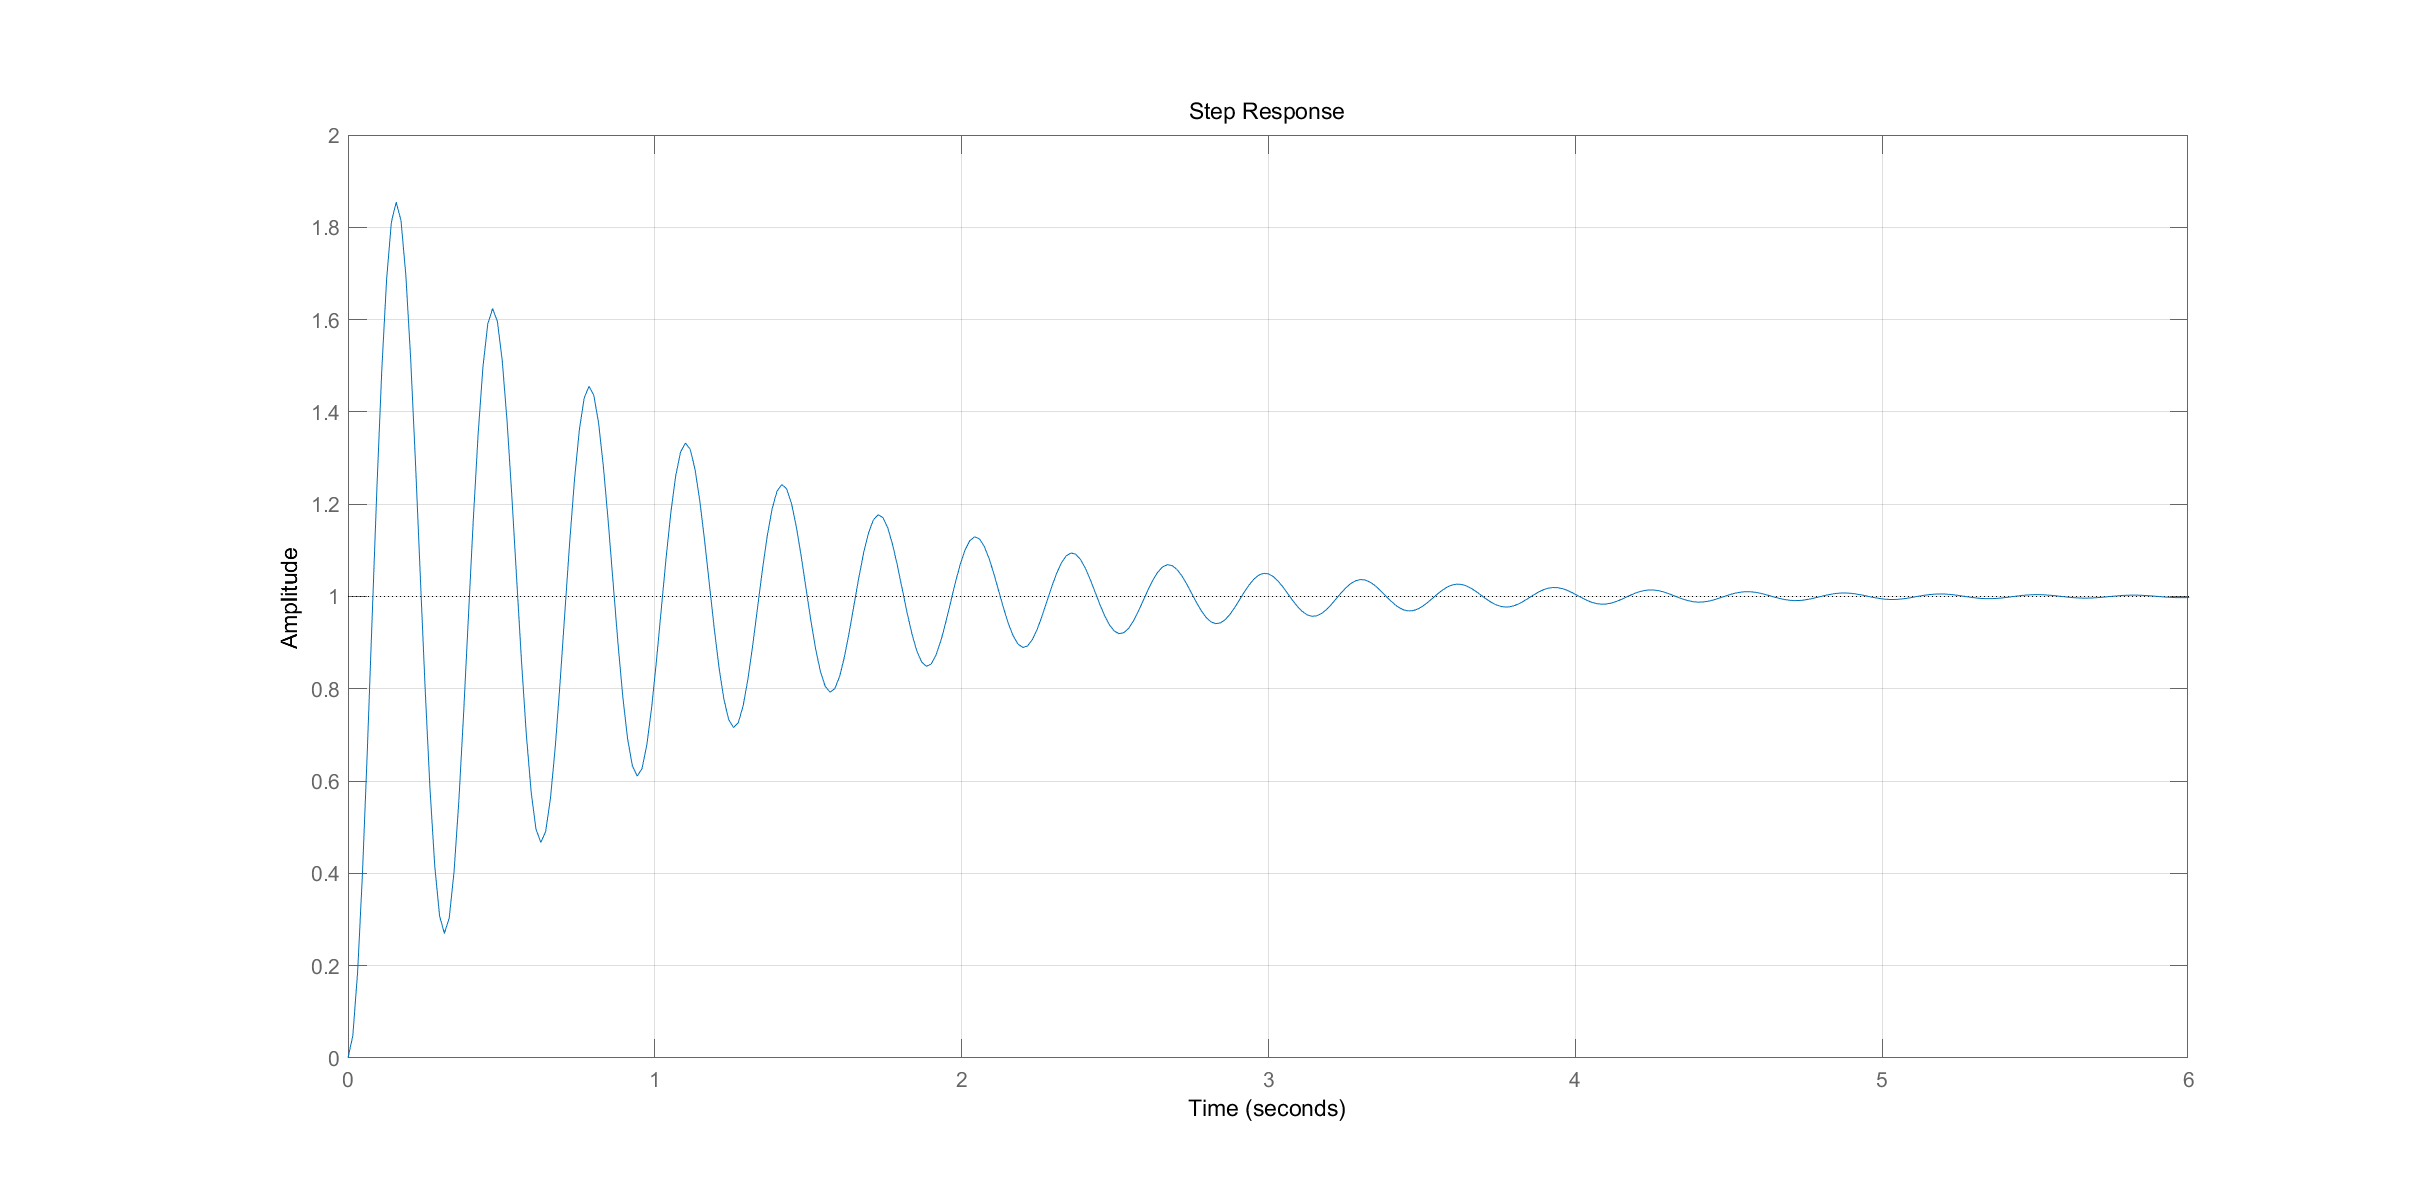
\includegraphics[width=1\textwidth]{3.1.3.eps}
    \end{center}
    \caption{3.1.3.}
\end{figure}
MATLAB Code:
\lstinputlisting{P3_1_3.m}

\end{document}